\begin{center}
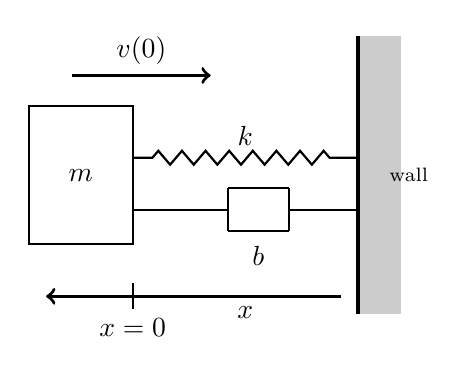
\begin{tikzpicture}[
    scale=1.1,
    spring/.style={thick, decorate, decoration={zigzag, pre length=0.25cm, post length=0.25cm, segment length=0.3cm}},
]
  % ---- wall ----
  \fill[gray!40] (4.2,0.4) rectangle (4.7,3.6);
  \draw[very thick] (4.2,0.4) -- (4.2,3.6);
  \node[font=\scriptsize, right] at (4.45,2.0) {wall};

  % ---- mass ----
  \draw[thick] (0.4,1.2) rectangle (1.6,2.8);
  \node at (1.0,2.0) {$m$};

  % ---- spring ----
  \draw[spring] (1.6,2.2) -- (4.2,2.2);
  \node[above=1pt] at (2.9,2.2) {$k$};

  % ---- damper ----
  \draw[thick] (1.6,1.6) -- (2.7,1.6);
  \draw[thick] (3.4,1.6) -- (4.2,1.6);
  \draw[thick] (2.7,1.35) -- (2.7,1.85);
  \draw[thick] (3.4,1.35) -- (3.4,1.85);
  \draw[thick] (2.7,1.35) -- (3.4,1.35);
  \draw[thick] (2.7,1.85) -- (3.4,1.85);
  \node[below=2pt] at (3.05,1.35) {$b$};

  % ---- velocity arrow (toward the wall) ----
  \draw[->, very thick] (0.9,3.15) -- (2.5,3.15) node[midway,above] {$v(0)$};

  % ---- x axis: x=0 at crash start, positive away from the wall ----
  \draw[->, very thick] (4.0,0.6) -- (0.6,0.6);
  \draw[thick] (1.6,0.45) -- (1.6,0.75);
  \node[below] at (1.6,0.45) {$x=0$};
  \node[below] at (2.9,0.6) {$x$};
\end{tikzpicture}
\end{center}
